\documentclass{article}
\usepackage{algorithm}
\usepackage{algpseudocode}
\usepackage[margin=1in]{geometry}
\usepackage{enumitem}
\usepackage{minted}
\usepackage{amsmath}
\usepackage{graphicx} % Required for inserting images

\begin{document}

     %\begin{center}
        % \fontsize{13}{15} \noindent \textit {Heaven’s Light is Our Guide}
     %\end{center}
    \begin{center}
        
\includegraphics[width=5cm]{RUET_logo.png}
    \end{center}
    
    
    \begin{center}
        \vspace*{0.2cm}
         \fontsize{15}{17} \bfseries {Rajshahi University of Engineering \& Technology}
         
        \fontsize{15}{17} \bfseries {Department of Computer Science \& Engineering}
        
       
    \end{center}
    
    \begin{center}
        \vspace*{0.2cm}
        \large{
        {\textbf{Course No :}  CSE 4204}
        
        {\textbf{Course title :} Sessional based on  CSE 4203}\\
         \noindent {Date : 04-12-2023}
         }
        \vspace*{2.2cm}
    \end{center}

    \begin{center}
        \fontsize{15}{17} \noindent {\textbf{Experiment No. : }}\large{03}
        \vspace{0.2cm}
    
        \fontsize{15}{17} \noindent {\textbf{Name of the experiment : }}\large{Design and Apply Multi-layer Neural Networks algorithm.}
        
        \vspace{1.4cm}
        \fontsize{15}{17} \noindent {\textbf{Submitted By :}}
        
        \vspace{0.2cm}
        \large{
        \noindent {Tanmoy Sarkar Pranto}
    
        \noindent {Roll : 1803166}
        
    	\noindent {Section : C}
    	
         \noindent {Dept. of Computer Science and Eengieering}
        
        \noindent {Rajshahi University of Engineering \& Technology}
        \vspace{1cm}
        }
        
        \fontsize{15}{17} \noindent {\textbf{Submitted to :}}
        \vspace{0.2cm}
        
        \noindent {{Rizoan Toufiq}}
        
        \noindent {Assistant Professor}
        
        \noindent {Dept. of Computer Science and Eengieering}
        
        \noindent {Rajshahi University of Engineering \& Technology}
    
        
        \vspace*{1.2cm}

       
    
        
    \end{center}

    \newpage
    \tableofcontents
    \newpage
    
    \vspace{0.5cm}


   \section{\fontsize{15}{17}{\noindent \textbf{Theory }}}
    \begin{flushleft}
        \noindent
        \large{
        The Multilayer Perceptron (MLP) is a fundamental building block of deep learning, capable of solving complex classification and regression tasks. \\ 
        \noindent  Here's a breakdown of its theory and key concepts:}



        \begin{enumerate}
            \item \textbf{Perceptron:}
                \begin{itemize}
                    \item The basic unit of an MLP is the perceptron, a simple neuron-inspired model.
                    \item It takes weighted inputs, sums them, and applies a threshold function to generate an output (0 or 1).
                \end{itemize}
            \item \textbf{Multilayer Architecture:}
                \begin{itemize}
                    \item MLPs go beyond single perceptrons by stacking them in layers.
                    \item The output of a layer becomes the input for the next layer, creating a chain of information processing.
                \end{itemize}

            \item \textbf{Activation Functions:}
                \begin{itemize}
                    \item Instead of a simple threshold, MLPs use non-linear activation functions to introduce complexity.
                    \item Popular choices include sigmoid, ReLU, and tanh, which allow the network to model diverse relationships beyond just linear ones.
                \end{itemize}

            \item \textbf{Learning and Backpropagation:}
                \begin{itemize}
                    \item MLPs learn by adjusting the weights connecting neurons based on their performance on training data.
                    \item Backpropagation compares the network's actual output to the desired output and propagates the error backwards through the layers, updating weights to minimize the error in future predictions.
                \end{itemize}

            \item \textbf{Loss function:}
                \begin{itemize}
                    \item Measures the error between network output and desired output (e.g., mean squared error).
                \end{itemize}
                
			\item \textbf{Learning rate:}
                \begin{itemize}
                    \item Controls how much the weights are adjusted based on the error.
                \end{itemize}
                
            \item \textbf{Advantages:}
                \begin{itemize}
                    \item \textbf{Versatile:} Handles various tasks like classification, regression, and pattern recognition.
					\item \textbf{Interpretable:} Can analyze learned weights to understand how the network makes decisions.
					\item \textbf{Efficient:} Relatively fast to train compared to other deep learning models.
                \end{itemize}

           \item \textbf{Limitations:}
                \begin{itemize}
                    \item Can struggle with high-dimensional data and complex problems requiring significant feature engineering.
					\item Prone to overfitting if not regularized properly.
					\item Requires careful hyperparameter tuning for optimal performance.
                \end{itemize}

        \end{enumerate}


  
    \end{flushleft}

    \section{\fontsize{15}{17}{\noindent \textbf{Algorithm}}}
    \begin{flushleft}


\large {
\textbf{Steps:}\\
\vspace{0.5cm}
1. Initialize weigths, biases and learning rate\\
2. Present inputs and desired outputs (dataset)\\
3. Calculate actual output\\
4. Calculate error\\
5. Adapt weights with backpropagation\\}
\end{flushleft}

    	 
    \vspace{0.5cm}
    

    \section{\fontsize{15}{17}{\noindent \textbf{Code}}}

    \begin{minted}{python}

import numpy as np
import matplotlib.pyplot as plt

epoch_losses = []

def sigmoid(x):
    return 1 / (1 + np.exp(-x))

def forward(X, W1, b1, W2, b2):
    z1 = np.dot(X, W1) + b1
    a1 = sigmoid(z1)

    z2 = np.dot(a1, W2) + b2
    a2 = sigmoid(z2)

    return a1, a2

def train(X, Y, W1, b1, W2, b2, epochs=3000, learning_rate=0.1):
    for epoch in range(epochs):
        A1, A2 = forward(X, W1, b1, W2, b2)

        E = Y - A2

        delta2 = E * (A2 * (1 - A2))

        delta1 = np.dot(delta2, W2.T) * (A1 * (1 - A1))

        W2 += learning_rate * np.dot(A1.T, delta2)
        b2 += learning_rate * np.sum(delta2, axis=0)
        W1 += learning_rate * np.dot(X.T, delta1)
        b1 += learning_rate * np.sum(delta1, axis=0)

        loss = np.mean(np.power(E, 2))

        if epoch % 300 == 0:
            print(f"Epoch {epoch}: loss = {loss}")
        epoch_losses.append(loss)

X = np.array([[0, 0, 0],[0, 0, 1],[0, 1, 0],[0, 1, 1],
    [1, 0, 0],[1, 0, 1],[1, 1, 0],[1, 1, 1]
])
Y = np.array([
    [0],[1],[1],[0],
    [1],[0],[0],[1]
])

W1 = np.random.randn(X.shape[1], 4)
b1 = np.random.randn(4)
W2 = np.random.randn(4, 1)
b2 = np.random.randn(1)

train(X, Y, W1, b1, W2, b2)

_, predictions = forward(X, W1, b1, W2, b2)
for i in range(len(predictions)):
    predictions[i] = predictions[i].round()
    
def calculate_accuracy(predictions, labels):
    correct_predictions = np.sum(predictions == labels)
    total_samples = len(labels)
    accuracy = correct_predictions / total_samples
    return accuracy


def plot_loss_curve(loss_values):
    plt.plot(loss_values, label='Training Loss')
    plt.xlabel('Epoch')
    plt.ylabel('Loss')
    plt.title('Epoch Loss Curve')
    plt.legend()
    plt.show()
    
accuracy = calculate_accuracy(predictions, Y)
print(f"Accuracy: {accuracy}")
plot_loss_curve(epoch_losses)


    }
    
    \end{minted}


    \vspace{1cm}
    \section{\fontsize{15}{17}{\noindent \textbf{Performance Analysis}}}
    \vspace{0.5cm}
    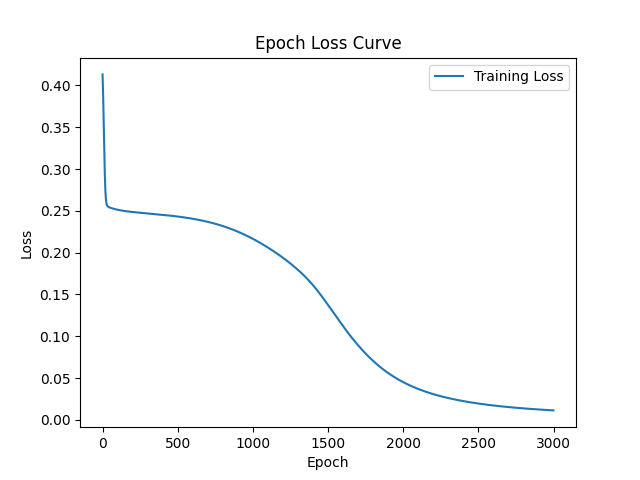
\includegraphics[width=15cm, height=10cm]{Figure_1.png}\\
    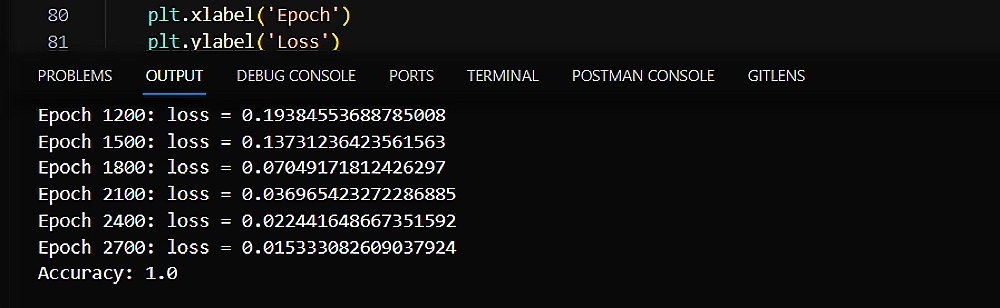
\includegraphics[width=15cm]{publication_ready_SS(142)_1.jpg}

    \section{\fontsize{15}{17}{\noindent \textbf{Discussion}}}

    \noindent The implemented Multilayer Perceptron achieved 100\% in the 3 bit X-OR dataset. From the epoch-loss curve we can see the curve starts around 0.4 initially and decreases rapidly. This suggests the model quickly learned basic patterns in the data. After nearly 2500 epochs the loss is nearly 0 (0.05), which means the model converges to the problem properly. Overall, the Multi Layer Perceptron successfully solved the X-OR problem. . 






\end{document}
